\documentclass{IEEEtran}
\usepackage{graphicx}
\usepackage{verbatim}
\usepackage{url}
\usepackage{color}
\usepackage{array}
\usepackage{multirow}
%\usepackage{subfigure}

%%%%%%%%%% verbatim related
\usepackage{fancyvrb}
\usepackage{fixltx2e}
\fvset{framesep=2mm,fontsize=\scriptsize,framerule=.1mm,numbersep=1mm,commandchars=\\\{\}}
\usepackage{listings}
\usepackage[usenames,dvipsnames]{xcolor}


%%%%%%%%%%%%%%%%%%

\newcommand{\eat}[1]{}
\newcommand{\rmv}[1]{ #1}
\newcommand{\sysname}{XXXXXX}

\newif\ifrev
% comment out the following line after the revision is done
\revtrue
\ifrev
  \newcommand{\cappos}[1]{{\color{red} [Justin: #1]}}
  \newcommand{\reznik}[1]{{\color{blue} [Leon: #1]}}
  \newcommand{\weiss}[1]{{\color{green} [Richard: #1]}}
 \newcommand{\yanyan}[1]{{\color{blue} [Yanyan: #1]}}
\else
  \newcommand{\cappos}[1]{}
  \newcommand{\reznik}[1]{}
  \newcommand{\weiss}[1]{}
\fi

\begin{document}

\title{Trust Evaluation in Mobile Devices: \\An Empirical Study}
\author{Leon Reznik$^*$, Richard Weiss$^{\star}$, Albert Rafetseder$^{\dag}$, 
Yanyan Zhuang$^{\dag, \ddag}$, Justin Cappos$^{\dag}$, ??\\
$^*$Rochester Institute of Technology, $^{\dag}$Evergreen College\\
$^{\dag}$New York University, $^{\ddag}$University of British Columbia}

\maketitle


\begin{abstract}
Trust evaluation of complex and diverse systems, such as an ad-hoc network 
of mobile devices, is a significant challenge in both theory and practice. 
In order to manage the complexity, we develop a hierarchical trust 
evaluation methodology that fuses trust evaluation metrics of individual devices 
and their components, and verifies and adjusts the overall trust evaluation 
based on the consistency of data from multiple devices.
  
%Smartphones  are rich in sensors and network easily with other mobile devices and wearable computers.

\eat{
  Smartphones and mobile devices install software from a 
wide range of sources.  As these devices become
more popular, the risks of associated malware will become more significant.
One of the features of these platforms is that they are rich in
sensors\footnote{In this work, smartphone sensors are broadly defined as hardware components that can record phenomena about the physical world.}.  These sensors can be a risk to privacy in that they could leak information about the 
user and user activities.  On the other side, they can also be used as an
advantage if they can be used to evaluate trust.
%leak information about any malware that is running on it.  
This paper builds  a hierarchical trust evaluation 
 framework 
that uses sensors to evaluate trust and detect anomalies.
} % end comment

The paper describes the hierarchical trust evaluation framework 
developed and tested for Android based smartphones. The 
framework operation involves two stages: initial trust evaluation 
based on the expert rules application, and the 
evaluation scheme verification and adjustment based on the analysis 
and comparison of data, which might be extracted from various mobile 
devices. We examine the results of two empirical studies, in which 
this framework is applied and tested. The first study involves 
monitoring resource utilization and evaluating trust based on 
resource consumption patterns. For example, malicious code injected 
into an app or OS utility typically results in an increased consumption of 
system resources, such as CPU or network communication. 
%Sensor values like battery level 
%and CPU utilization can detect this.  The second study uses a comparison of erroneous sensor values
%from the GPS sensor on a smartphone with speed data from the OBD port on an automobile.
%These are examples in which malware could produce an intentional or inadvertant effect on sensors, such 
%ass GPS receivers or a speedometer, and could be detected by measuring anomalies 
%in these sensor values. 
The second study involves verification of the trust evaluation by 
comparing the measurement results coming from the smartphone 
GPS location sensors against an external speedometer sensor in a car.
\eat{
Our approach is two-fold: evaluating trust based on metrics 
and models, \yanyan{more specific what the metrics and models are?} and 
using this evaluation to detect anomalies as a way to improve security in general.} % end comment

\eat{For many people, smartphones and other mobile devices serve as a technical interface to the modern world.
These smart devices have embedded on-board sensors, such as accelerometers, gyroscopes, GPS sensors, and
cameras, which are very useful.

This work describes \sysname, a hierarchical framework for checking consistency of sensors 
from multiple devices.  In addition, it relies on Blursense, a dynamic, fine-grained, flexible access
control mechanism, acting as a line of defense that allows users to define and addprivacy filters. 
As a result, the user can expose filtered sensor data to untrusted apps, and researchers can collect 
data in a way that safeguards users' privacy.}  %end comment
\end{abstract}

%\IEEEpeerreviewmaketitle

\section{Introduction}

Android-based mobile devices and smartphones are becoming increasingly popular.  The number of mobile phones
sold has surpassed the number of laptops, reaching 1.3 billion in 
2014~\cite{market}.  Google is 
reported to have more than a billion active users of 
Android-based devices~\cite{android-users}.  
As their popularity increases, so does their value as
a target for malware.  
This is particularly true for low cost smartphones sold in developing countries. According to \cite{zheng2014droidray}
some vendors there intentionally create conditions facilitating various security violations on these devices.
 There are many possible risks associated with using compromised devices.  Nowadays due to universal interconnectivity and 
interdependence between devices and networks, the 
possible compromise of a mobile device will affect not only applications on it and its users, but all other 
networked computers and communication infrastructure.
\eat {There are many possible risks.
Many people use smartphones for financial transactions. 
 Attackers could get personal information for systems administrators and CIOs from their phones and 
 use that for spear phishing.  mention security and privacy issues}  % end comment
With the development of the mobile communication platforms that share different devices resources, applications and data, 
vulnerabilities and security threat will become more wide-spread. 

In order for mobile devices to communicate with each other and download apps securely,
they need to be able to compute trust metrics.   Trust can be modeled at 
multiple levels, e.g. at the application level, on a device (hardware and software), or among a network of devices.  Ultimately, our goal
is to integrate these metrics into a single conceptual framework so that we can reason about complex systems at a  
higher level, and we can also use them to verify trust for individual components.
The trust evaluation  could 
be applied to optimize data collection and communication schemes in order to satisfy multiple criteria such as 
data quality, overall
system performance and/or resource consumption, subject to the constraints based on security and privacy requirements.
Also, the user of a device may benefit from the trust evaluation as it might 
provide useful information about areas in need of improvement. The trust evaluation could also be combined with other techniques for
 non-signature based intrusion detection.

The more sophisticated mobile devices become, the more complex the threat model is, and the more opportunities there 
are for vulnerabilities to appear.  Trust evaluation should be sensitive to the detection of viruses and other 
malicious agents in a system.
However, finding viruses and other malware using software signatures is less likely to
work.  Signature based intrusion detection systems have to be complemented with a system-wide  approach that 
involves assessing trust for the different
components by detecting anomalies in sensor-originated data.
\eat{
In recent research done by Hoffman, the authors developed a hierarchical 
mechanism that is scalable and expandable for evaluating security of
Android smartphones by investigating various sources of information regarding 
the mobile devices. 
The three sources of information that they integrate are:
analysis of installed applications using metadata provided by the Google Play store,
usage information coming from security tools embedded in the OS, and 
validation of the device by inspection of sensor data.  
The sensors in this context refer to any function that
measures the physical state of the smartphone.  This can include geolocation, accelerometers, CPU 
utilization, and battery charge.} % end comment


\eat{
- McKnight and Chervany, What is Trust? A Conceptual Analysis and an Interdisciplinary Model
- Paul England, Butler Lampson, John Manferdelli, Marcus Peinado, Bryan Willman: A
Trusted Open Platform. IEEE Computer Scciety, p55-62, July 2003.
- Adrian Baldwin, Simon Shiu: Hardware Security Appliances for Trust. In Proceedings of
the First International Conference of Trust Management (iTrust 2003), Crete, Greece, May
2003.
- Daniel W. Manchala: Xerox Research and Technology. E-Commerce Trust Metrics and
Models. IEEE Internet Computing, vol.4, no.2 p.36-44 (2000).
- Mui Lik, Mohtashemi Mojdeh, Halberstadt Ari: A Computational Model of Trust and Repu-
tation. In Proc. Of the 35th Annual Hawaii International Conference on System sciences, 7-
10 (Jan. 2002), Big Island, HI, USA.
- Mogens Nielsen,  Karl Krukow A Bayesian Model for Event-based Trust, 2007
- Zheng Yan and Piotr Cofta, “A Mechanism for Trust
Sustainability among Trusted Computing Platforms", In Proceedings of the 1st
International Conference on Trust and Privacy in Digital Business
(TrustBus2004), LNCS Vol. 3184/2004, pp. 11-19, Spain, September 2004.
} % end comment

The concepts of trust and trust evaluation have been discussed by many others~\cite{jing2014riskmon,shabtai2010google,zheng2014droidray}; 
however, it seems that the problem  of quantification is largely unsolved, especially with respect to complex systems.
 Yet, the nature of our work points to ways in which 
this could be used to produce secure or trustworthy systems.  
This paper presents the development of the novel hierarchical model that enables the  evaluation of trust for a 
network of mobile devices. Trust evaluation depends on numerous factors. The hierarchical or umbrella structure allows for the
inclusion of various trust evaluation systems used to assess diverse trusted components as well as their integration 
in order to produce a cumulative trust score. Also, it allows for extending the framework by inclusion of new trust 
metrics and facilitates both self-evaluation for a particular device as well as the collaborative evaluation of 
diverse devices and applications. 
The paper describes the version developed for Android-based devices.

The rest of this paper is organized as follows. 
Section~\ref{sec-umbrella} describes the framework design principles and an overall architecture. Also, this section 
 briefly describes a few of the trust evaluation metrics developed for individual apps and
smartphones that are included in the current implementation.
Details about a few of the trust evaluation metrics are provided in Section~\ref{sec-iheart}--\ref{sec:geolocation}. In particular, Section~\ref{sec-iheart} discusses metrics 
for individual apps based on measuring resource utilization such as battery voltage, CPU and network bandwidth usage,
which can be done on the smartphone.
Section~\ref{sec:blursense} describes metrics based on multiple sensors that impact the level of privacy supported, and how 
privacy-enhancing tools can interact with trust evaluation.
Section~\ref{sec:geolocation} discusses the possible ways in which trust evaluation can be verified and adjusted, based on multiple sources
of data. We show that data collected simultaneously from a smartphone and on-board diagnostics (OBD) 
sensor of an automobile can be used in trust evaluation.
 % this will describe the problem and applications, threat models
\section{FRAMEWORK UMBRELLA ARCHITECTURE AND DESIGN}
%This is a summary of section 2 in the Hoffman paper

\begin{figure*}[t]
\centering
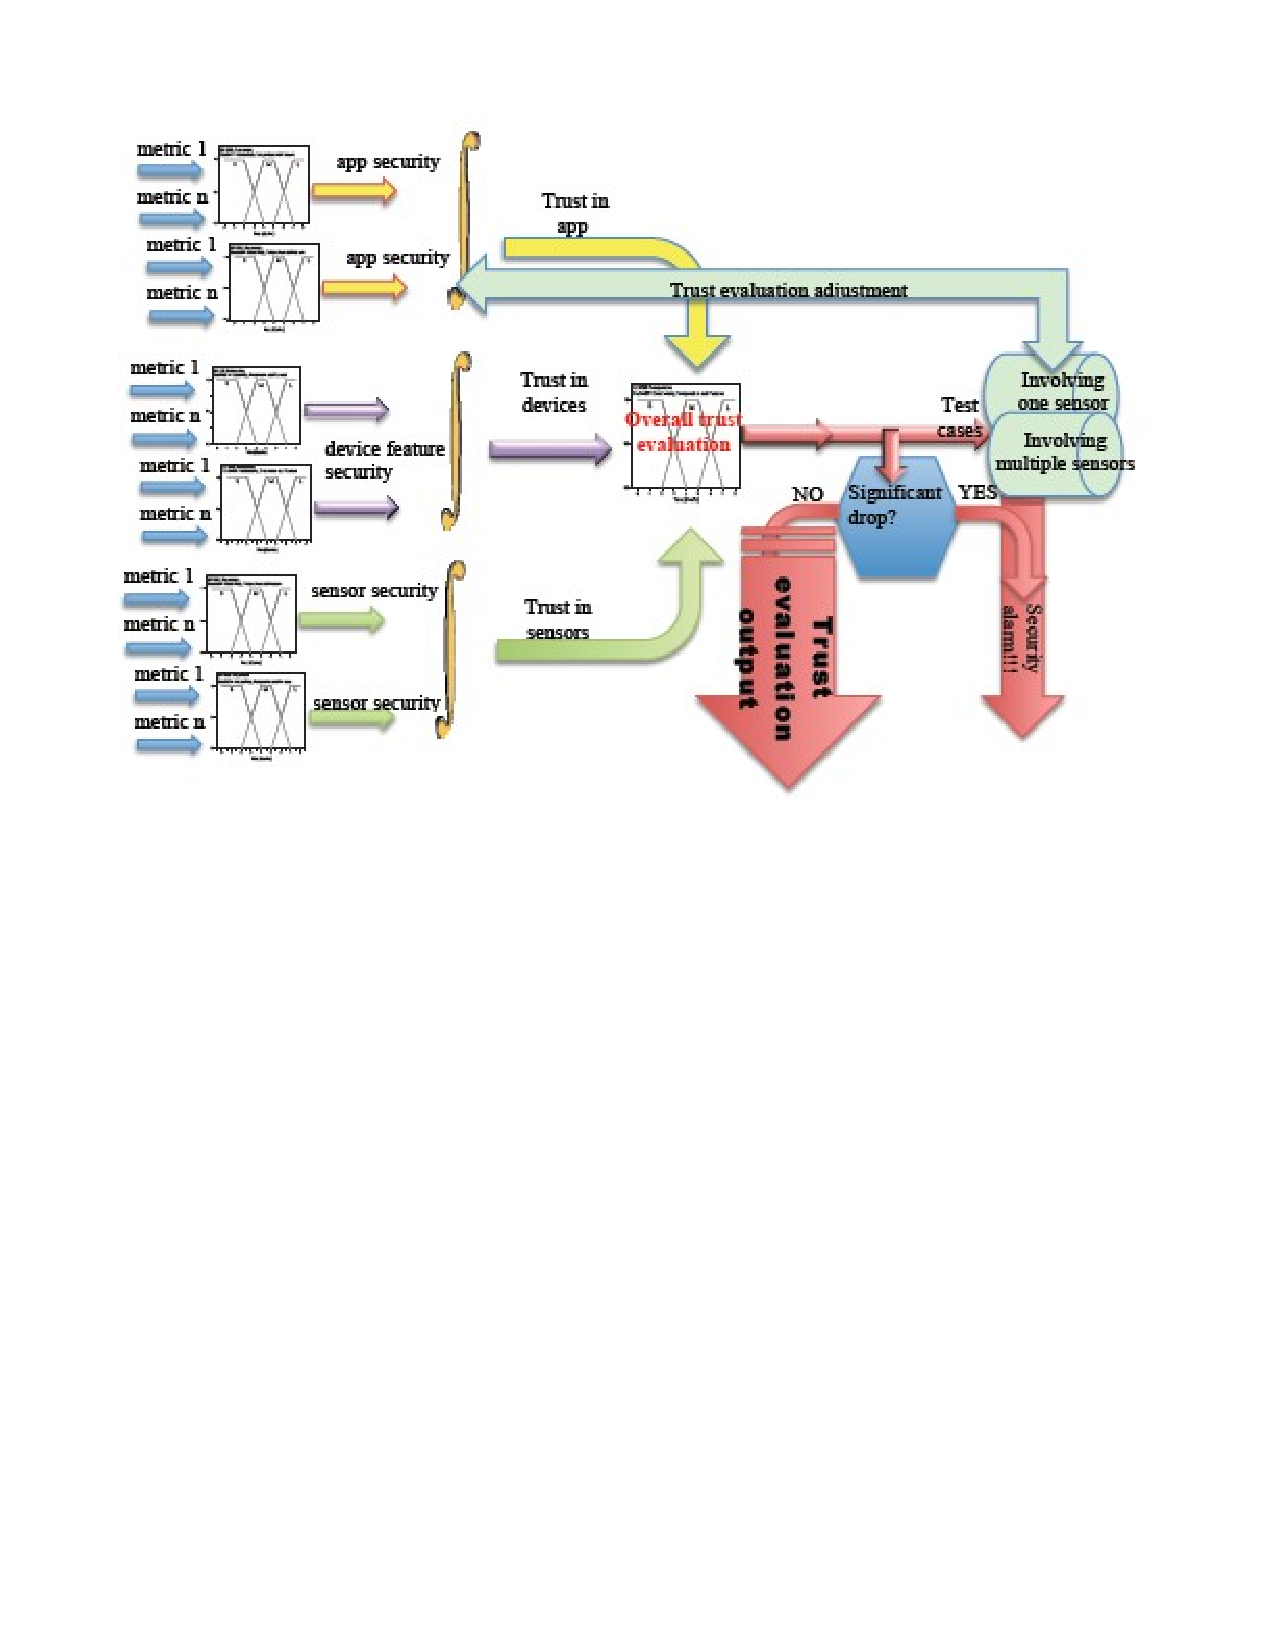
\includegraphics[width=7.0in]{umbrella_framework.pdf}
\caption{Framework operation and architecture.}
\label{fig:umbrella}
\end{figure*}

A hierarchical trust analysis can look at the entire system and combine measurements from multiple sources, making
it more powerful than measuring a single component or layer.
This section discusses a comprehensive mechanism that provides a scalable and extendable methodology of trust
 evaluation and analysis which is implemented on Android-based mobile devices. \weiss{why is it limited to Android?}
Trust evaluation of a mobile smartphone device is a complex subject, which depends on multiple characteristics, 
e.g. sensor accuracy, the rate of encrypted messages, \weiss{I don't understand that one}
 and/or the probability of a system's breakdown over a given period of time. Its evaluation should integrate various metrics ranging from the accuracy and reliability of the data sources to the security of the procedures and tools used. The major research challenge of the framework design is integrating the numerous metrics needed to characterize a device's trustworthiness while working with limited resources and processing power. 
We address this challenge by hierarchically structuring the composition of trust metrics as well as by designing a specialized calculus to evaluate the overall trust metric. 
Therefore, the major innovative emphasis in our framework design is put on the integration of a wide variety of indicators and their evaluation procedures. The framework procedures output the overall trust evaluation indicators and additionally calculate the individual product of metrics characterizing system features which are then used to produce recommendations for improvement. The trust evaluation will facilitate decision-making, improve performance and increase accountability through the collection, analysis, and reporting of relevant performance-related data. This design facilitates the framework extension through
 the inclusion of other metrics, as well as the ease of modification and improvement (see fig~\ref{fig:umbrella})
Current implementation of this framework provides the following metric functionality: 

\begin{enumerate}
\item Analysis of the installed applications through the application-specific metadata provided by the Play store. Applications represent the largest security and privacy risk to a device and user's data. The data provided by the Play store leverages the experiences of millions of users and holds all data associated with the distribution of an application including its associated documentation. The Play store also provides meta-information about applications which gives useful characteristic data about an application. These data can be used to assess an individual application's risk. Rules were generated to classify each application into a risk impact class based on this meta-data. The combined trust classes of all applications installed on a device would be used to create a security risk rating for the whole device.

\item The usage verification of security tools embedded into the operating system and proper preventative security practices. Android provides users with many different tools which increase the security and privacy of their devices in addition to updates 
to patch exposed vulnerabilities.  When properly used, these tools improve the security of the devices. They are 
intended to gather a 
comprehensive overview of the software running on a mobile device by analyzing the operating system and user settings. 
First the operating system is checked to confirm that it is running the most recent version available. Second the personal 
security settings on the device are examined to determine if the user is utilizing the appropriate tools to secure the device. 
These operating system verification checks combined generate a score, which is used in the security and privacy framework operation result.

\item The trust evaluation based on the level of privacy provided.  
The spurious output of a device's internal sensors can sometimes indicate the existence of a privacy/security problem 
%Verifying the validity of the sensors can detect security and quality problems of the device 
that would be missed by the other metrics. Most mobile devices now come equipped with a variety of sophisticated 
internal and external sensors which are capable of very accurate measurements of their surrounding environment. 
As the data from these sensors are used in more security critical applications the importance that these data remain accurate and legitimate should not be underestimated. For example, data from the GPS sensor can be verified to be trustworthy and assigned a trust rating. The combination of ratings from all sensors would produce the devices sensor trust score.
% privacy: disclosing the user's exact location.  Users have only very coarse-grained control
% an app that uses Google map service would most likely request this in the manifest file.
\end{enumerate}


Unlike other reported tools available, our framework has an umbrella structure that allows for integration of 
diverse trust evaluation mechanisms and results through a rule-based classification system.
This open architecture can also be extended to include 
 self-learning capabilities to allow for its optimization towards a particular device and a criteria set. Each of these procedures given above generates a security risk rating, which is then integrated into the umbrella framework. This framework takes into account the varied landscape of mobile devices and is designed to be flexible and easily adaptable to the changing security environment. Based on this design and contribution of each of the procedures could be adjusted depending on the target.

\subsection{Rule-based Classification}
The goal is to assign a trust level to an application based on usage patterns (this is a part of the
overall trust evaluation hierarchy).
The classifications are: 
\begin{enumerate}
  \item Low trust: These applications are considered to have
a low trust evaluation and a high probability of its negative
impact on the overall device security
  \item Moderate trust: These applications are evaluated to have
less negative  impact on the overall device security
  \item High trust: These applications are considered to have a high
trust evaluation or a low probability of  negative impact
on the overall device security.
\end{enumerate}

We evaluate overall trust based on a separate
analysis of each application. On the first step the list of all
applications installed on the device is compiled. After that the
manifest file for each application installed is analyzed in order to
fetch the application name, package name, required features,
version, required permission, path info, date on which the
application was installed and the target SDK version. This
information is used to evaluate  trust according to the classification.
However, this is refined using
application category. This information could
be retrieved from the Google Play store. The Google Play store
holds all data associated with the distribution of an application
including its APK file and associated documentation.  Following
features can be retrieved from the
meta-data:
\begin{itemize}
  \item Number of Installs – Total number of installs across the apps life
  \item Number of Reviews – Total number of reviews from unique users
  \item Score – User rating of 1.0 to 5.0
  \item Developer – Name of the developer
  \item Permissions – Which resources can be accessed by the app
\end{itemize}

The first three fields can be used to find an application’s
popularity which when matched with a history of values shows
user trend information.  Although it may not be possible to determine if an
application is a security risk based on this
information, data from a large number of users could be very reliable~\cite{}.

it can be used in rules in combination with other data~\cite{jing2014riskmon}.

Here are some examples of rules that are used in the classification: 
\begin{itemize}
  \item If number of downloads were low with low ratings, the
    application was classified as low trust.
  \item If the number of downloads were low with good application
    score, the application was classified as moderate trust.
  \item If the application had low recent score it was classified as moderate trust
    stating that there was something wrong with the latest patch released by the developer.
  \item If the application was from a unknown publisher with low score
    and low number of downloads it was classified as low trust.
  \item If the application was from an unknown publisher with high
    number of downloads and high score it was classified as moderate trust.
\end{itemize}
 % summary of section 2 of the Hoffman paper
\section{Measuring app behavior}

Anomalous behavior of a smartphone may be due to malicious adulteration of an application,
the operating system, or the hardware during the manufacturing chain.
In order to be able to detect this
behavior, we first need to establish baseline measurements for 
normal behavior. We focus on metrics that are observable 
without requiring inspection of the app's source or binary code
because obfuscation techniques are very sophisticated and will continue to be developed.
We have enhanced existing debugging techniques with additional internal sensor measurements to inspect app behavior.
Aggregate metrics, such as battery voltage, CPU usage, and network usage are easy to collect.  
Because they measure different components of the system, they can be considered as independent with
respect to trust metrics.  On the other hand,
they can also be influenced by random and extraneous factors unrelated to trust.

\subsection{Battery voltage}
The battery voltage is a proxy metric for the amount of remaining 
energy in the battery. Any kind of activity on the device will result 
in a change of battery voltage, but the resolution of readings (both 
in time and in voltage) only allows for coarse, averaged measurements 
under general, non-lab conditions.
If the circumstances can be controlled tightly, then approaches like 
\textit{Eprof} \cite{pathak2012fine} can be used to estimate energy consumption 
of individual activities and assign credit to likely originators.  In the following experiment,
the battery voltage was measured both with and without ads.
The ​baseline is the battery consumption playing  music.
This was recorded for 15 seconds, 60 seconds, and 10 min.  Then, the measurement was repeated
with both video ads and the music app.  The video ads were only running for the first 15 seconds.
The smartphone consumes only 31.5mA with no apps running, and 56.5 mA with the radio app
running.
But when playing a video ad, the consumption is 169.5mA. 
In the experiment, the video ad lasted 15 seconds.
Over the first 15 seconds, the average battery use attributed to the video ads was 81\% of the total
battery use.  This is very significant and would be difficult to disguise.
The data are shown in table~\ref{table:battery}



\begin{table}[ht]
\centering 
\scriptsize
\begin{tabular}{|l|l|}
  \hline
  {} & {Rate of consumption(mA)} \\
  \hline
  {} & {31.5}\\
\end{tabular}

\begin{tabular}{|l||l|l|l|}
    \hline
    {\bf Time} & {\bf 15s} & {\bf 60s} & {\bf 10min} \\
    \hline
    \% of total battery use with ads (avg)  & 81.4\%   & 53.0\%   & \\
    \hline
    \% of total battery use with ads (max) & 86.0\%  & 61.5\%  & 11.9\%  \\
    \hline

\end{tabular}
\caption{A comparison of battery use with anomalous adware compared with normal.
The ad was 15 seconds.}
\label{table:battery}
\end{table}

\subsection{CPU usage}

\begin{figure*}[ht]
\centering
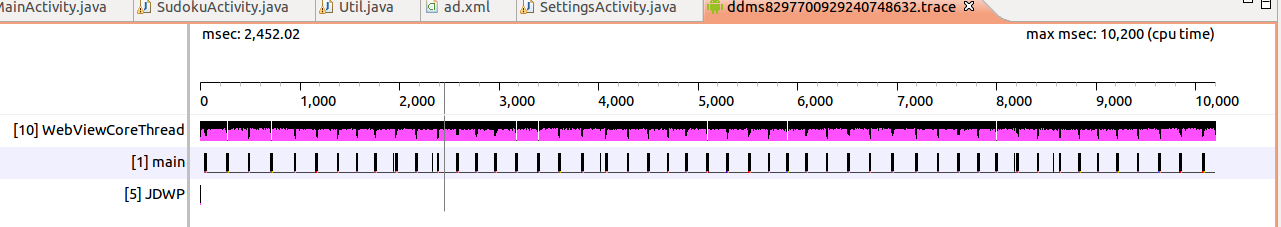
\includegraphics[width=6in]{no_AdsDisplay_10s.png}
\caption{A typical session in Traceview, the execution log viewer.
WebViewCoreThread is busy, but main thread's workload is very light.  main is reponsible for 
the user interface, in general.  WebView is reponsible for rendering ads using the webkit library}
\label{fig:cpu-no-ad}
\end{figure*}

\begin{figure*}[ht]
\centering
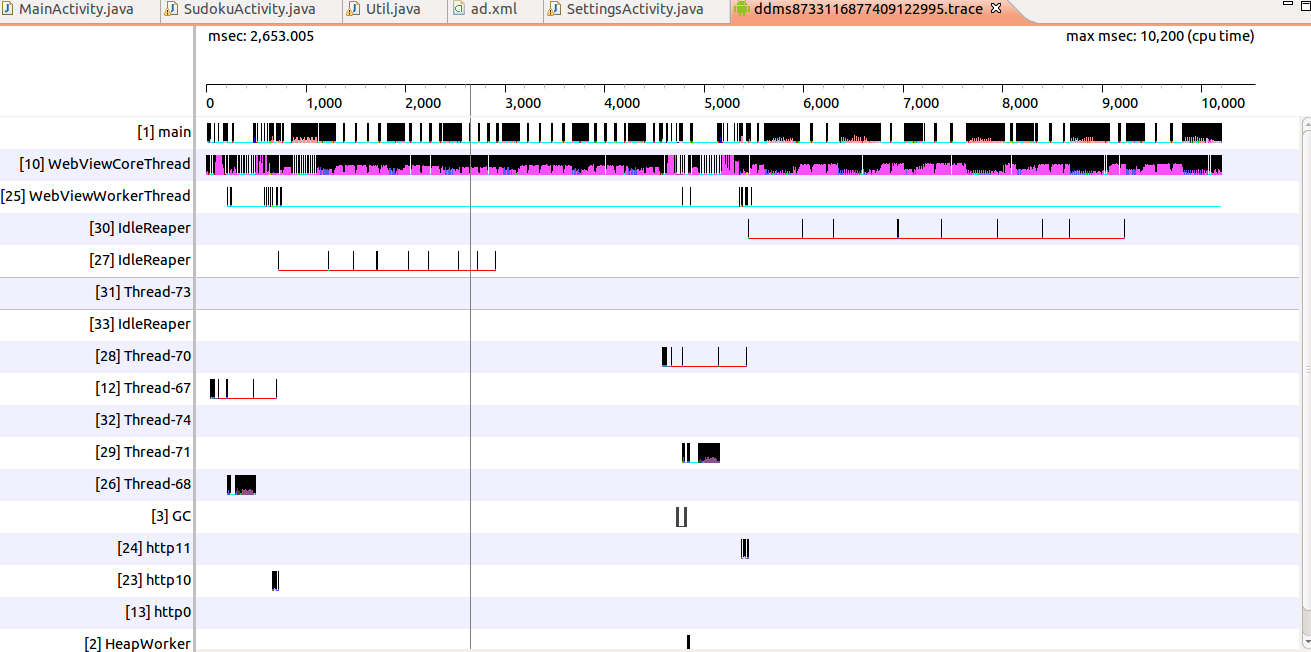
\includegraphics[width=6in]{traceview.png}
\caption{A session in Traceview, with anomalous Ads.  Notice that main is doing much more work and
there are other threads that are getting significant CPU time.}
\label{fig:cpu-ad}
\end{figure*}

Similar to battery voltage, monitoring the overall CPU usage 
(which is an operation requiring no special privileges on Android) 
can be used to get a coarse-grained overview of resource utilization. 
However, the existing debugging and tracing interfaces permit 
finer-grained views as well. Assuming an app is not designed to 
evade or complicate debugging deliberately, the 
\textit{Dalvik Debug Monitoring Service} (DDMS) 
% https://developer.android.com/tools/debugging/ddms.html
provides syscall-level insight.  \weiss{Even if an app is trying to evade reverse engineering,
 would it be hard to eliminate the frequency of syscalls?}

Figure~\ref{fig:cpu-no-ad} shows a typical  
session in Traceview, the execution log viewer.  The main thread is doing almost all of the work
and making system calls.  Figure~\ref{fig:cpu-ad} shows what happens when a video ad starts 
executing.  There is a dramatic change in activity and the main app thread is no longer 
the primary, uniform consumer of CPU cycles.
% Current figure (MD5 46fbce842e071dfb8f321c9645c6b411) courtesy of Tao Li.
The app under scrutiny comprises several threads with different 
temporal activity patterns. Some threads bear names indicative 
of their performed functions. Colored bars in the threads' activity 
timelines further detail call-level interactions with app and system 
libraries, with the height of sub-bars proportional to the frequency 
of specific calls.  
Other log views (not shown) list all of an app's threads, show the 
call stack for each, and display cumulated and individual CPU time 
consumption, and relative usage.


%%% http://www.sigmobile.org/mobisys/2012/program.php#ses5

\subsection{Network usage}

Android provides a number of built-in features allowing the observation 
of a device's network conditions for any app granted the 
\texttt{ACCESS\_NETWORK\_STATE} permission. 
The \texttt{ConnectivityManager} class lets an app discover the 
current connectivity status and type (WiFi, 3G, Bluetooth, Ethernet)~\cite{che2011case}. 
For cellular access such as LTE or 3G, the \texttt{TelephonyManager} 
class makes available further detail. The stateful nature of cellular 
data connectivity is reflected by various indicators of data activity, 
thereby allowing any app to detect when other apps transfer data over 
the cellular interface.  The Application Resource Optimizer project
(ARO\footnote{See \url{https://github.com/attdevsupport/ARO}}) and \cite{Ricciato2010551} 
provide further insights into what is 
essentially radio resource control (RRC-based type of diagnostics).

%%% https://developer.android.com/reference/android/telephony/TelephonyManager.html (See NETWORK_TYPE_* and DATA_* states)
%%% https://developer.android.com/reference/android/net/ConnectivityManager.html (See TYPE_*)
%%% https://developer.android.com/reference/android/net/NetworkInfo.html#isConnected%28%29

If the device is \textit{rooted} (i.e., system-level administrator 
privileges are available to the user launching an app), standard 
packet tracing tools such as \texttt{tcpdump} can be used to 
record the exact data transferred across network interfaces. 
However, the precondition is not met on almost any commercial stock 
firmware.
% Note: tcpdump doesn't allow inspection of encrypted content either. 
% There are approaches adding a system-level certificate to MITM on 
% HTTPS connections see for instance https://github.com/egirault/googleplay-api ,
% but I think this also requires root.

When packet-level tracing on the device is infeasible, the network 
connection of the device might be tapped instead. A natural place 
for this would be a WiFi router acting as the device's gateway. 
Neither on-device nor on-path packet tracing allow decryption of 
HTTPS and other encrypted network traffic. However, at least for 
HTTPS implementations using the system libraries, deliberate 
man-in-the-middle (MITM) attacks on traffic may be performed 
by adding a self-provided certificate to the system's certificate 
storage, and redirecting outgoing HTTPS traffic to a local proxy 
server using that certificate.
  % what is anomalous behavior, how are resources monitored?
\section{Trust Evaluation Metrics Based on The Supported Privacy Level}
\label{sec:blursense}
Privacy is part of trust evaluation.
The greater the level of privacy that an application or device can provide, the greater its trust evaluation would be.
A privacy enhancing system such as BlurSense~\cite{cappos2014blursense} can improve the trustworthiness of an Android device  
 by filtering or restricting the sensor data that an application can access.
In addition,
one can apply trust metrics to automate the application of Blursense itself.  For example, if an app has a low trust evaluation,
then BlurSense can restrict the sensor data that the app has access to.

\subsection{Motivation}
Although the sensing capabilities enhance the convenience of user interfaces and
application usefulness, they also raise serious privacy
concerns~\cite{shabtai2010google}. For instance, through accessing sensor data,
malicious applications could retrieve sensitive information about the mobile
phone users, such as location, passwords, and credit card numbers~\cite{xu2012taplogger, 
miluzzo2012tapprints, xu2009stealthy, cai2011touchlogger}. They
even might be able to send sensitive information to remote
attackers~\cite{schlegel2011soundcomber, marquardt2011sp}. There
has been alarming news about privacy breaches of personal data on smart devices:
25\% of Android apps in Google Play can access user's personal
data~\cite{toomuch}; an iOS app can auto-post false piracy accusations on users'
Twitter accounts~\cite{tweetios}; apps could steal sensitive information like
passwords using the smartphone's motion sensors to determine key 
taps~\cite{xu2012taplogger}; and a huge botnet was discovered that was collecting sensor data
on more than a million end user smartphones~\cite{botnet}. The
Federal Trade Commission (FTC) even recommended that mobile platforms should
provide in-time disclosures to users of accessing sensitive content on smart
devices~\cite{ftc}. 

\subsection{Applying Trust Metrics to BlurSense}
Trust metrics can also be used by privacy enhancing tools such as BlurSense to limit access to sensor data.
The current access control to the smartphone resources,
such as sensor data, is static and coarse-grained. 
%However, such defense is pre-determined by the manufacturer. 
Take the
Android platform as an example, the access permissions are
either granted or denied completely during the installation of
applications based on a request XML manifest file. As a result,
applications may ask for more permissions than are actually
required for operation. Having been granted the requested
permissions, applications have access to those resources permanently. 
A trust metric could be used during installation of an app to decide whether or not
to deny access specified in its manifest file.  
A better approach is to restrict access to sensor data in a
dynamic and fine-grained framework.
Some systems that have been proposed to address this
issue require modifications to the Android
platform~\cite{conti2011crepe, hornyack2011these}. This increases the cost of maintenance, is
less flexible and cannot be used in legacy systems. In addition,
the user would need to trust that the new operating system is
not malicious and is not more vulnerable than the standard one.

\begin{figure}%[htd]
  \centering
  % Requires \usepackage{graphicx}
  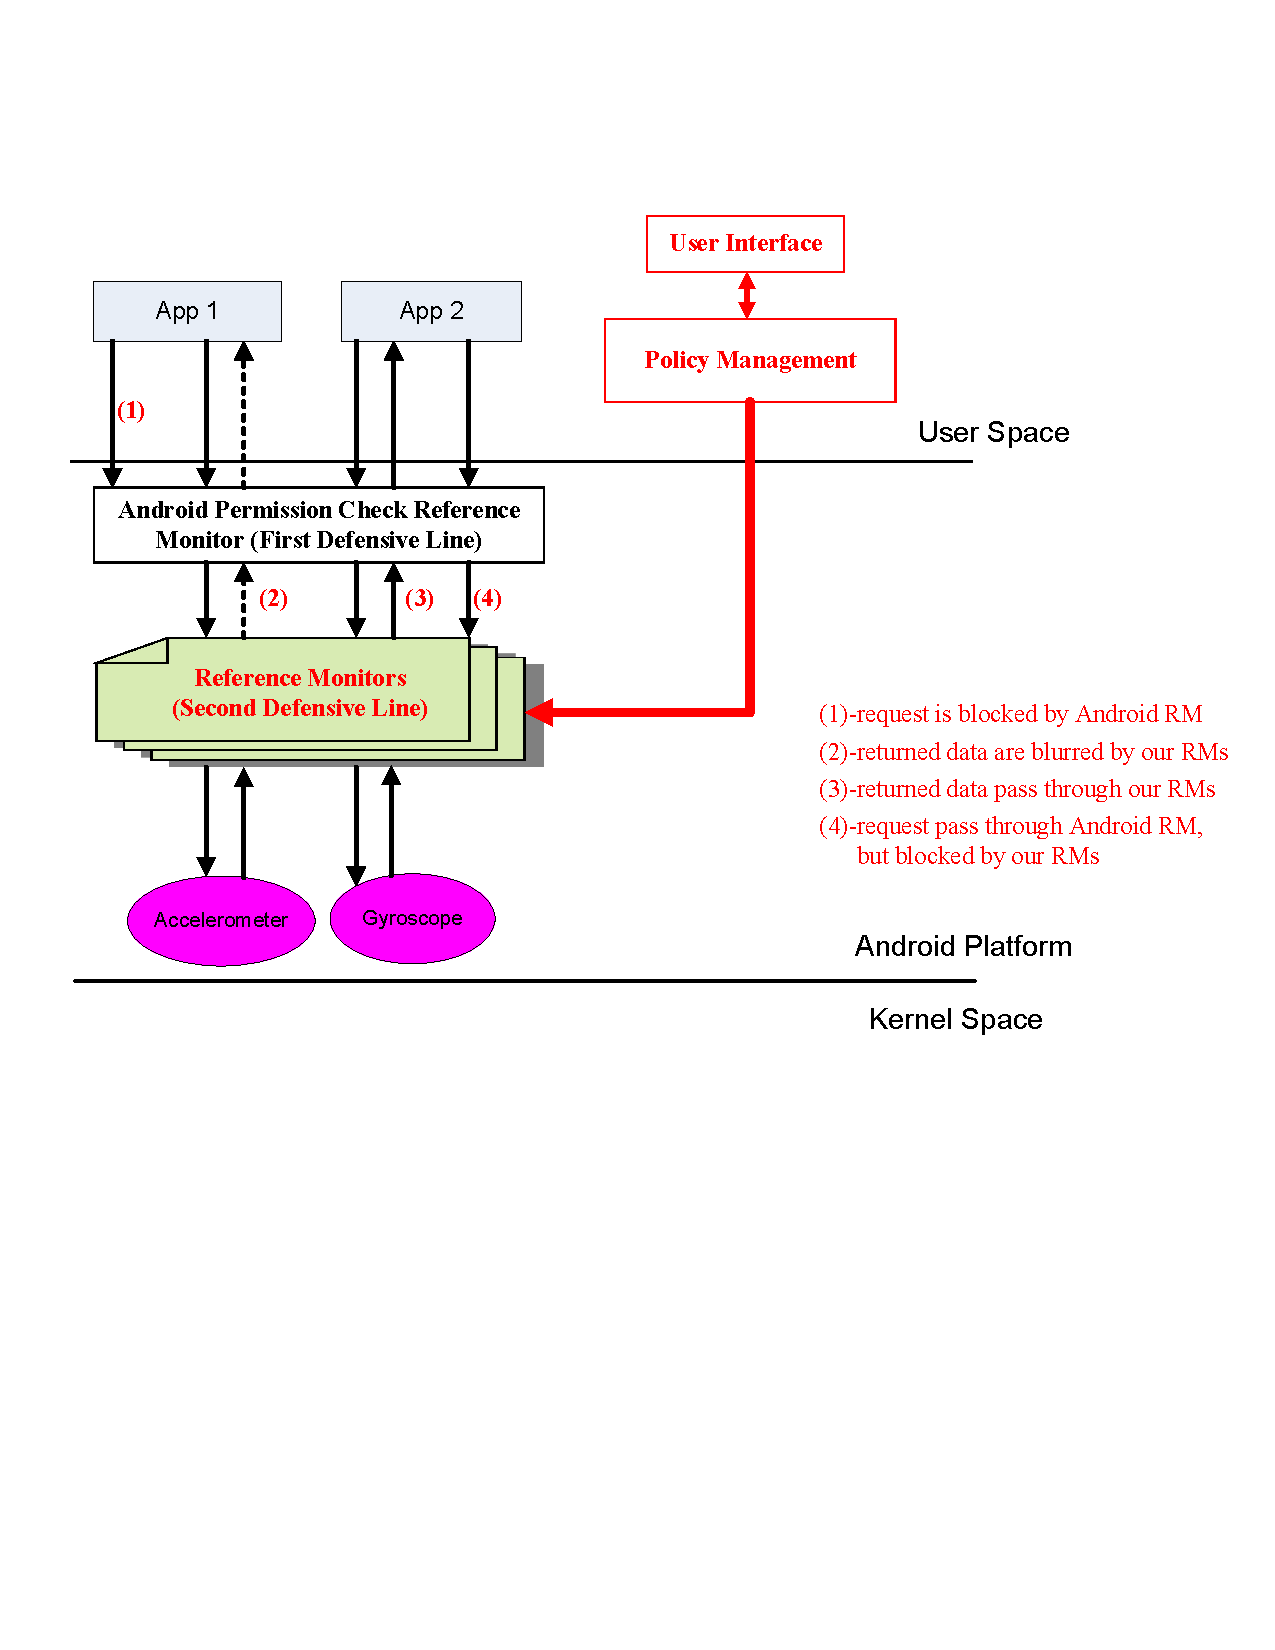
\includegraphics[width=3.7in]{refMonDesign.pdf}\\
  \caption{System architecture based on reference monitors.}
  \label{Fig:design}
\end{figure}

The BlurSense project deals with this problem of fine-grained conrol of sensor data
by requiring that all untrusted apps be installed
through an app that filters sensor data through a reference monitor~\cite{cappos2014blursense}.  
(See Figure~\ref{Fig:design})
The policy for filtering can be set by the user based on a trust metric.
 The reference
monitor can exercise fine-grained control to degrade the accuracy of the sensor data, render it 
completely meaningless, or pass it through unchanged.  
In the case of geolocation, GPS measurements can be set to the center of the nearest
large city or random noise can be added.  Another approach would be to allow the user to decide
whether to in stall the app or not, based on the trust evaluation 
%based on the sensor data requested in the manifest file.
The reference monitor approach poses less risk than others; the worst that can happen is
that the app will have the same access to the sensor data that
is permitted by the manifest file. In the best case, BlurSense
would limit the access to sensor data based on a combination of trust metrics for the app.
BlurSense is currently able to filter data on battery level, CPU usage, geolocation (latitude, longitude,
altitude, accuracy, and speed if available), and network related measurements
(mobile network type and operator, nearby WiFi access point
and Bluetooth devices).

\eat{
Currently, implemented sensor modules and
the available contextual information are classified into three
categories: device specific (percentage of battery power level,
CPU and memory utility), location related (latitude, longitude,
altitude, accuracy, and speed if available), and network related
(mobile network type and operator, nearby WiFi access point
and Bluetooth devices). While sensor modules are the system
hooks with read access to valuable sensor resources, they
cannot manipulate sensor data. Additionally, the sensor API
also provides a base registry service with a common interface
for use by a sensor implementation. } % end comment
\eat{For both local and remote
processes to access sensor data, a JSON/sl4a library
is incorporated to provide data in an unified format. In case
newer sensors appear on future mobile devices, developers can
add newly implemented sensors into this framework rather
easily. 
%The registry service listens for connection on a set of predefined ports via XML-RPC. 
Thus, both local and remote
process can connect to these ports and register for sensor
updates.
Our preliminary work in this area has resulted in working 
code~\cite{seattle-sensor-git}, tutorials~\cite{seattle-sensor-project}, and a 
blog for problem discussion~\cite{sensor}. Several different groups have
already used our early-stage proof-of-concept to solve problems across a variety
of domains, demonstrating the potential of sharing sensor data. 
} % end comment

  % description of the experiments: comparisons of driving data
\section{Measuring geolocation behavior}
%Description of the OBD system, how data can be retrieved from the car.
Another form of verification is the use of sensors on multiple devices.  For example,
a smartphone may communicate directly with a smartwatch or on-board diagnostics (OBD)
sensor on an automobile.  These other devices have sensor with the same
functionality as some of the sensors on the smartphone.
% describe what data is collected, how it is stored, and how it might be used.
% we can include a graph of spped error vs time and the picture of the car route
We introduce a case where smartphones communicate with an in-vehicle OBD sensor
to get geolocation information, such as speed, engine RPM, fuel consumption, 
etc.

\subsection{Vehicle data collection}

Our vehicular data collection consists of a process on a mobile 
device that directly communicates with in-vehicle sensors and collects sensor 
data~\cite{sensor}. Data can be encrypted and transferred to our 
centralized server for permanent data storage. \weiss{we should put a diagram of 
the data collection and storage}
To depoly such a process on a mobile device, a device owner first installs an
app~\cite{sensor-app} on their devices\footnote{Currently, Android smartphones 
and tablets are supported.}. Since we are interested in
vehicular data, the target group of device owners are also vehicle 
owners. These owners simply insert their WiFi On-Board Diagnostics 
(OBD)~\cite{obd} sensor into their cars' OBD ports (located under the steering wheel),  
%\linda{I don't think they insert their sensor into the car. Do they insert it into something specific in the car (e.g., a usb port)? That would make sense. Anyway, I think you need to be more specific in stating what gets connected to what} 
and connect their 
smartphone or tablet to the sensor, which also runs as a WiFi access 
point. Note that OBD systems are in most cars and light trucks 
on the road today~\cite{obdconnector}. Therefore, our 
infrastructure does not require extra installation of specialized  
hardware or equipment~\cite{reininger2015first}. 

A person interested in getting vehicular data uploads his  
code to run in the background of the mobile device, and to communicate 
with an in-vehicle OBD sensor to get vehicle data. Device owners need not worry about having to
interact with the app or about being interrupted as they use their smartphones. 
Note that all code runs in a secure sandbox in our 
app~\cite{sensor-app}, which limits the amount of storage, network, 
memory, battery, and CPU resources used by any code~\cite{Cappos_CCS_10}. 
To protect end users' devices from malicious attackers, the sandboxed 
code is securely isolated from other programs on the same device.
Any bugs in the code will be contained in the sandbox, and will not 
affect the rest of the user device~\cite{Cappos_CCS_10}. 
%Once our prototype data collection application is installed and running on an Android smartphone with Sensibility, the end user need not worry about interacting with a user interface on the Android. Rather, once the user inserts their WiFi OBD sensor into the car and connects their Android smartphone to the sensor running as a wifi access point, our 
%

At the remote server, the vehicular sensor data collected from 
multiple end user devices is stored in a non-relational database. 
An example of 
collected data is shown in Figure~\ref{fig:json}, in JSON format.
The collected data set can be visualized on Google Maps to 
identify fuel efficient routes, routes with higher traffic activity, and routes 
(and drivers) that exhibit a high frequency 
of reckless or illegal driving behaviors, etc. 

\begin{figure}
\scriptsize 
\begin{Verbatim}
\{
  \textbf{"sensors"}: \{
    \textbf{"speed_car"}: \textcolor{red}{60},
    \textbf{"maf_car"}: \textcolor{red}{4},
    \textbf{"rpm_car"}: \textcolor{red}{114},
    \textbf{"gps_phone"}: \{
      \textbf{"error"}: \textcolor{red}{null},
      \textbf{"id"}: \textcolor{red}{0},
      \textbf{"result"}: \{
        \textbf{"network"}: \{
          \textbf{"time"}: \textcolor{red}{1407200660927},
          \textbf{"speed"}: \textcolor{red}{60},    
          \textbf{"altitude"}: \textcolor{red}{4.099999904632568},
          \textbf{"bearing"}: \textcolor{red}{82.6999694824219},
          \textbf{"provider"}: \textcolor{OliveGreen}{"gps"},
          \textbf{"longitude"}: \textcolor{red}{-73.986706},
          \textbf{"latitude"}:\textcolor{red}{40.694010},
          \textbf{"accuracy"}: \textcolor{red}{7},
        \}
      \}
    \},
    \textbf{"id"}: \textcolor{OliveGreen}{"310410696731709"},
    \textbf{"time"}: \textcolor{SkyBlue}{"ISODate"}(\textcolor{OliveGreen}{"2014-08-05T21:04:07.183-04:00"})
\}
\end{Verbatim}
\caption{JSON document of vehicular data.\label{fig:json}}
\end{figure}

\subsection{Data store}
Given the variety of sensors on a smartphone,
sensor measurements come in different forms. 
As shown in Figure~\ref{fig:json}, many types of sensor data have complex structure.
As a result, we decided to use a non-relational database, 
MongoDB~\cite{mongodb}, for storing sensor data. MongoDB has a Binary 
JSON (BSON) document-style structure identical to that shown previously 
in Figure~\ref{fig:json}, albeit converted into binary as its name suggests. 
This provides the scalability that is crucial to our system and that allows dynamic storage of 
new sensors, as needed. 

\subsection{Geolocation data analysis}

\begin{table}
\scriptsize
\centering
\begin{tabular}{|p{.06\columnwidth}|p{.18\columnwidth}|p{.22\columnwidth}|p{.28\columnwidth}|}
\cline{2-4}

%\multirow{3}{*}{Statistics}

\multicolumn{1}{c|}{}  & \textbf{GPS speed} & \textbf{Vehicle speed} & \textbf{Speed difference}  \\ \hline

% Mean & 5.559 & 1.568 & 0.003606 \\ \hline 

Med & 53.0~kph & 54.9~kph & 2.15~kph \\ \hline

STD & 12.79~kph & 13.61~kph & 4.57~kph  \\ \hline

\end{tabular}
\caption{\small Speed comparison: GPS speed comparing to OBD speed.}
\label{tab:speed-diff}
%\vspace*{-15pt}
\end{table}

\begin{figure}
\centering
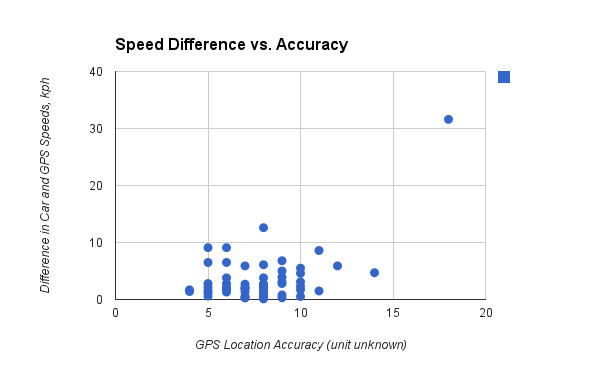
\includegraphics[width=3.5in]{speed.png}
\caption{Speed difference and accuracy.}
\label{fig:speed-diff}
\end{figure}

Using the aforementioned measurement, we collected speed data from both GPS 
on the smartphone inside a vehicle, and the speed via the OBD sensor. 
The data from these two sources can corroborate to verify normal or abnormal 
geolocation data. Table~\ref{tab:speed-diff} shows the median and standard deviation
of the speed measured by GPS and OBD sensor, over 58 data samples collected. 
The overall statistics do not show any anomaly in speed. However, when plotting 
individual data samples, we can see a data outlier in Figure~\ref{fig:speed-diff}. 
Excluding this point, the rest of the data samples roughly follow a Gaussian 
distribution. This outlier could be due to an error in vehicle 
OBD sensor, or due to an error injected into the code. \yanyan{please fix this}


\begin{figure}
\centering
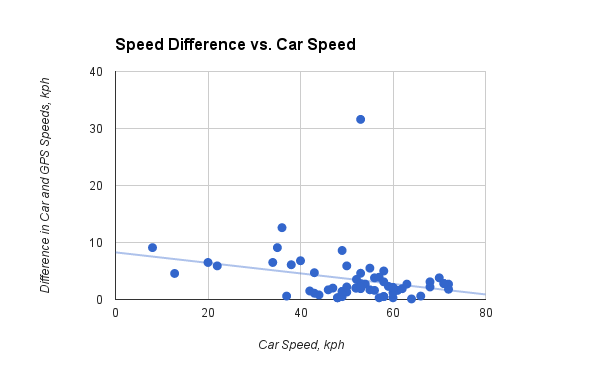
\includegraphics[width=3.5in]{car.png}
\caption{A typical session in Traceview, the execution log viewer.}
\label{fig:car}
\end{figure}

To further investigate on the speed data, we plot the differences between 
vehicle speed and GPS speed, and compare the differences against 
the varying vehicle speed. As shown in Figure~\ref{fig:car}, the speed 
differences are in a linear relation with the vehicle speed 
(other than the outlier), i.e., the 
higher the vehicle speed, the smaller difference between vehicle 
speed and GPS speed. \yanyan{any other observations?} 
The linear relationship in the figure is based on minimum mean 
square error (MMSE) xxx. \yanyan{please fix this}

\begin{figure}
\centering
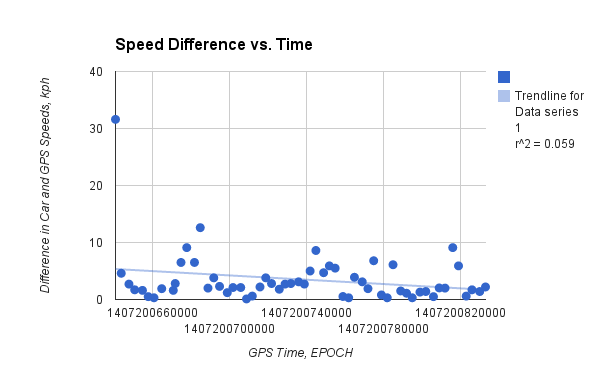
\includegraphics[width=3.5in]{time.png}
\caption{A typical session in Traceview, the execution log viewer.}
\label{fig:time}
\end{figure}

We also investigate the speed differences over time. 
In Figure~\ref{fig:time}, we can conclude that excluding the outlier, 
the differences between 
vehicle speed and GPS speed fluctuate around a constant value over 
time. The result is based on MMSE xxx. \yanyan{please fix this}
 % summary of sensibility platform with some blursense added and
            %  description of the OBD system
%\section{Results}
  
\section{Conclusion}
With the growing number of mobile devices owned by ordinary citizens all around the world and an increase of their participation in the network traffic generation and data provided, the problem of an evaluation of the trust, which other collaborators may have in the quality and security of their data and devices becomes more and more important. The presented trust evaluation framework includes procedures and tools to evaluate trust in mobile devices and applications, in particular in Android based smartphones. The framework hierarchical structure allows for incorporating multiple diverse factors affecting trust evaluation as well as facilitates its extension.
The current framework version includes the evaluation procedures based on the analysis of the following factors: the content of applications installed and executed, the device’s operating system settings and configuration, level of privacy supported by the devices and applications, patterns of the battery drain and CPU and network bandwidth usage. The conducted empirical study demonstrated a significant difference between the change of voltage in the cases of an execution of normal applications and the same applications with embedded additions, such as for example advertising. Another study produced distinguished patterns of the CPU and network use.
The framework includes not only the procedures of the trust evaluation but also the methods of its verification. 
Trust verification and adjustment could be performed through comparison of data received from different data sources on the 
same device as well as by comparing the data originated from various devices. The significant discourse between data 
originated from various sources should results in decreasing trust assessment for the corresponding data sources and devices. 
In the paper, we have described a comparative study of the speed measurements obtained from a car speedometer sensor and the speed calculated 
with the GPS location sensor measurements. This illustrates how the framework could be employed not only for trust evaluation 
but also for detecting various anomalies, which might include malicious attacks against the mobile devices.



% \section*{Acknowledgment}
% Weiss was supported by the National Science Foundation through grant TUES-1141341 
% Cappos was supported by the National Science Foundation through grants 

\bibliographystyle{abbrv}
\bibliography{bibdata,trust}

\end{document}

